\subsubsection{Entrenamiento de una red}\label{training}
Como resumen de visto hasta ahora, para crear una red es necesario tener cuatro elementos distintos:
\begin{itemize}
\item Valores de entrada: Información con la que se va a predecir un dato o un conjunto de datos.
\item Estructura de la red: Esta es una información que se debe de conocer a priori antes de crear el modelo. Tiene distintas propiedades:
\begin{itemize}
    \item Número de capas: A mayor número de capas, mayor será el tiempo que tardará el modelo en computar el vector de salida $y$ porque mayor cantidad de cálculos tendrá que realizar. El número de capas junto con el número de neuronas por capa son parámetros importantes, puesto que un número muy bajo en el modelo y este no tendrá una buena precisión. Por lo contrario un número muy alto puede producir lo que se conoce como \textit{overfitting}(ver sección \ref{overfitting}).
    \item Número de neuronas en cada capa: Cabe destacar que el número de neuronas en la última capa será el tamaño del vector $y$, es decir, el número de etiquetas que el modelo predecirá.
    \item Función de activación por cada capa.
    \item Arquitectura de la red. % Se puede ver más información sobre los tipos de arquitecturas de redes en la sección TODO.
\end{itemize}
\item Las matrices $W$: Son matrices que recogen la información asociada a cada capa sobre los pesos $w$ y \textit{bias} $b$ de cada neurona de la red.
\end{itemize}

Las matrices $W$ son matrices con valores creados aleatoriamente. El proceso de entrenamiento de la red tratará de optimizar estas matrices para que el vector $y$ resultante sea lo más preciso posible. Para poder entrenar un modelo es necesario tener previamente un \textit{dataset} con un conjunto de vectores $x$ y su valor real. La cantidad de datos que proporcionemos al modelo para que aprenda está relacionada con la precisión del modelo. Con el ejemplo descrito en la Tabla \ref{tab:houses} se podrían usar las columnas \textit{tipo}, \textit{coords}, \textit{gc}, \textit{m2} y \textit{h} para predecir el valor $precio$.
\newline

Básicamente la red inicializa la matriz $W$ de forma aleatoria. El modelo dado un vector $x$ realiza todos los cálculos de cada neurona y devuelve un valor $y$. $y$ es lo que el modelo ha predicho. Este proceso es el que se conoce como \textit{forward-pass}.
\newline

Para que la red aprenda, necesita primero saber si se ha equivocado y la magnitud del error. Si la magnitud de este error es muy grande, se deberá ajustar los valores de $W$ para minimizar el error. Por lo contrario, si el error es pequeño, no se ajustarán mucho los valores de $W$ porque realizando un ajuste en $W$ puede provocar una ligera mejoría en dicha predicción, pero puede desajustar otras predicciones que el modelo ha hecho previamente y eran también bastantes precisas. La elegancia de este algoritmo es que encuentra un balance entre lo que es ajustar valores para que la red aprenda y al mismo tiempo no desajustar demasiado para que la red se descompense en su aprendizaje global. Es la aplicación de la imitación del aprendizaje humano, un error con una gran repercusión deberá modificar comportamientos futuros, un error sin repercusión podrá ser ignorado o incorporar cambios proporcionados a las repercusiones.
\newline

El error se cuantifica con una función llamada función de coste o función de pérdida explicada en la sección \ref{costfunction}. A partir del valor del error, se usará un algoritmo que tratará de calcular la responsabilidad de cada neurona en dicho error y de esta forma poder ajustar los pesos y la \textit{bias} asociadas a dicha neurona. Este algoritmo se llama \textit{backpropagation} y es explicado en la sección \ref{backpropagation}.
\newline

Se puede pensar que este proceso se puede repetir infinitamente hasta tener un modelo perfecto, pero como se ve en la sección de \ref{overfitting} esto puede provocar que la red memorice el dataset que es usado para entrenar y no tenga la capacidad de generalizar. Por lo tanto, no solo se trata de ejecutar el algoritmo, sino que hay que realizar ciertas optimizaciones y tener varios conceptos en cuenta como por ejemplo: la selección de función de activación, diseño del vector de entrada y salida, métricas a usar, entre otros.
\newline

\label{p:company_backpropagation}
Como analogía para entender el algoritmo de \textit{backpropragation}, se puede usar la jerarquía de una empresa. Dicha empresa tras un trimestre desastroso elabora un resumen con los resultados. Estos resultados son equivalentes al error que el modelo produce. El jefe (la última capa de la red), tratará de rendir cuentas con los directivos. Estos directivos a su vez tratarán con otros directivos con menor responsabilidad y estos a su vez lo harán con jefes que estén por debajo suya y así sucesivamente hasta llegar al último nivel en la empresa (propagando el error hacia las capas más básicas). Posteriormente, la empresa elaborará un informe estudiando la responsabilidad de cada persona en el resultado del trimestre (que en el algoritmo de \textit{backpropagation} es conocido como el vector gradiente). Ese informe llegará al departamento de recursos humanos y este, tratará de modificar el comportamiento de cada trabajador en la empresa en función de su responsabilidad en el error (algoritmo del descenso del gradiente).
\newline

En el siguiente diagrama se puede visualizar el proceso que se lleva a cabo para entrenar una red neuronal: 
\begin{figure}[H]
    \centering
    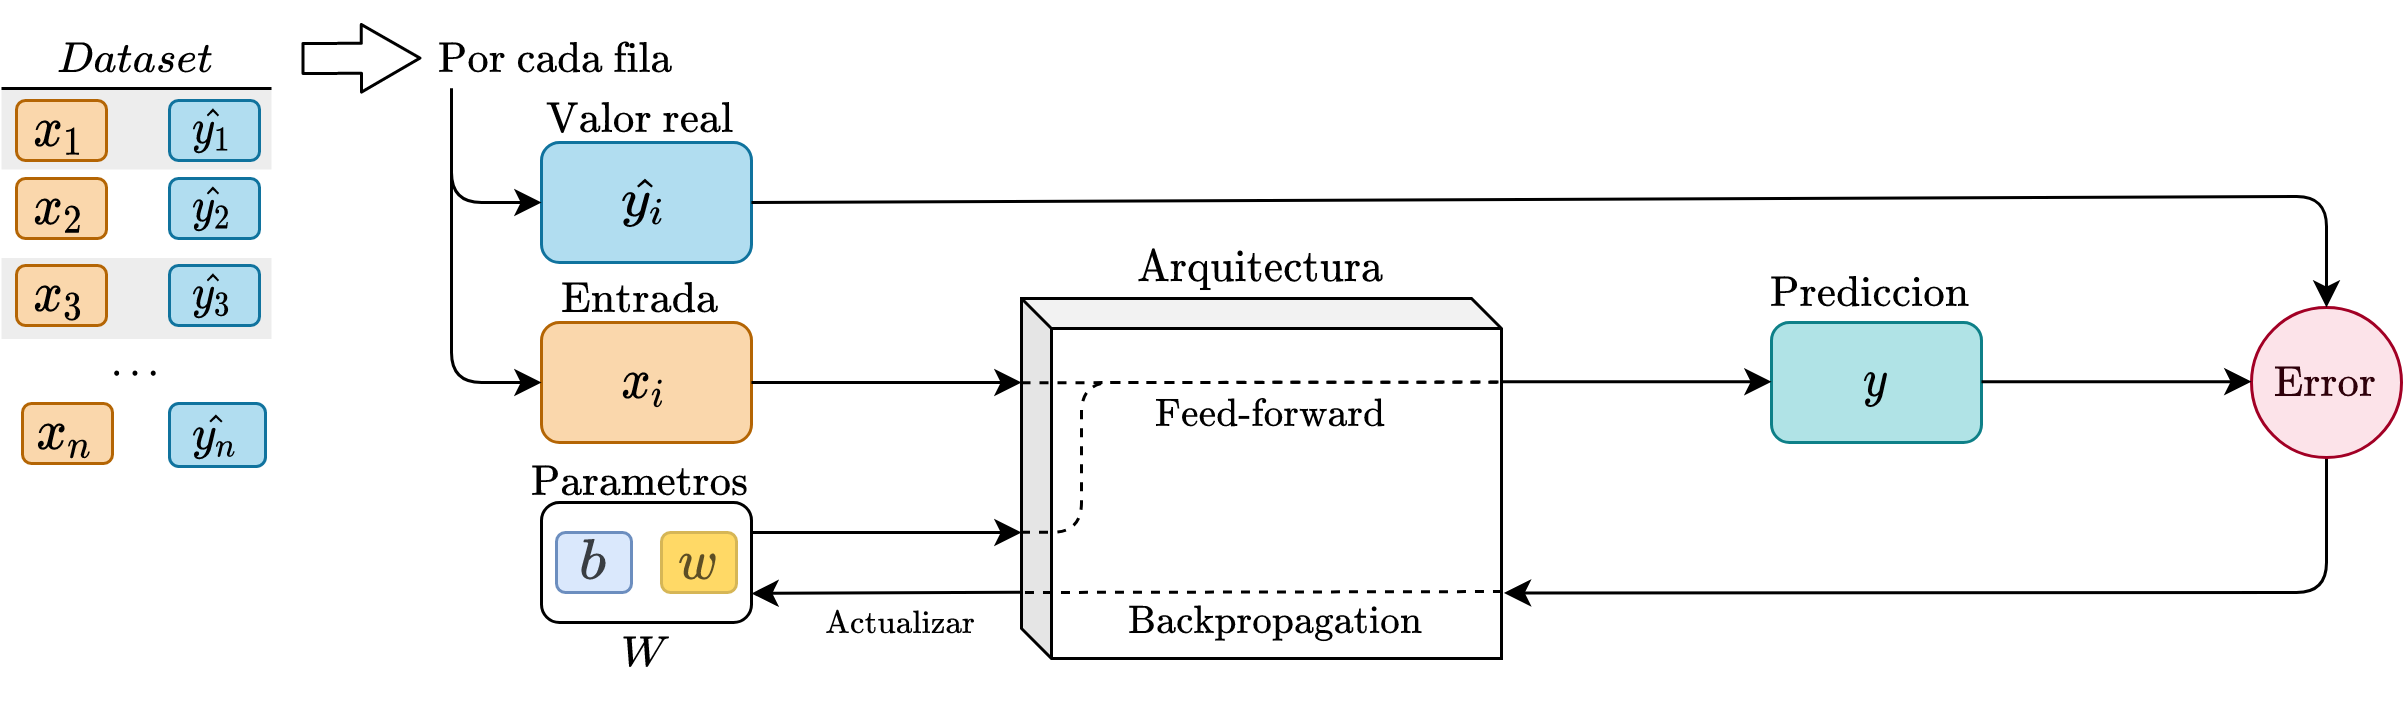
\includegraphics[width=15cm]{images/state-of-art/training/training.png}
    \caption{Proceso de entrenamiento de una red neuronal}
    \label{fig:error_regression}
\end{figure}

El entrenamiento de una red es un proceso iterativo. En cada iteración, o también conocido como \textit{epoch}, se tomarán un conjunto de datos del \textit{dataset} de entrenamiento de forma aleatoria. Cada uno de estos conjuntos de datos tomados para cada epoch se le denomina \textit{batch} y el tamaño del \textit{batch} suele ser un parámetro puesto por el usuario. El tamaño de un \textit{batch} suele ser de 32, 64 o 128 valores.
\newline

En cada \textit{epoch}, el modelo solo trabajará con dichos datos. Predecirá un valor para cada una de las entradas y junto al valor real, la función de coste, el algoritmo de \textit{backpropagation} y el descenso del gradiente, se irán ajustando de forma iterativa las matrices $W$.
